\documentclass{beamer}
\usepackage{amssymb,amsmath}
\usepackage{graphicx}
\usepackage{url}
\usepackage{color}
\usepackage{pagenote}[continuous,page]
\usepackage{relsize}		% For \smaller
\usepackage{url}			% For \url
\usepackage{epstopdf}	% Included EPS files automatically converted to PDF to include with pdflatex

%For MindMaps
% \usepackage{tikz}%
% \usetikzlibrary{mindmap,trees,arrows}%

%%% Color Definitions %%%%%%%%%%%%%%%%%%%%%%%%%%%%%%%%%%%%%%%%%%%%%%%%%%%%%%%%%
%\definecolor{bordercol}{RGB}{40,40,40}
%\definecolor{headercol1}{RGB}{186,215,230}
%\definecolor{headercol2}{RGB}{80,80,80}
%\definecolor{headerfontcol}{RGB}{0,0,0}
%\definecolor{boxcolor}{RGB}{186,215,230}

%%% Save space in lists. Use this after the opening of the list %%%%%%%%%%%%%%%%
%\newcommand{\compresslist}{
%	\setlength{\itemsep}{1pt}
%	\setlength{\parskip}{0pt}
%	\setlength{\parsep}{0pt}
%}

%\setbeameroption{show notes on top}

% You should run 'pdflatex' TWICE, because of TOC issues.

% Rename this file.  A common temptation for first-time slide makers
% is to name it something like ``my_talk.tex'' or
% ``john_doe_talk.tex'' or even ``discrete_math_seminar_talk.tex''.
% You really won't like any of these titles the second time you give a
% talk.  Try naming your tex file something more descriptive, like
% ``riemann_hypothesis_short_proof_talk.tex''.  Even better (in case
% you recycle 99% of a talk, but still want to change a little, and
% retain copies of each), how about
% ``riemann_hypothesis_short_proof_MIT-Colloquium.2000-01-01.tex''?

\mode<presentation>
{
  \usetheme{CambridgeUS}
  \usecolortheme{dolphin}
  \useoutertheme{default}
  \useinnertheme{default}
  \setbeamercovered{invisible} % or whatever (possibly just delete it)
}
\beamertemplatenavigationsymbolsempty

\usepackage[english]{babel}
%\usepackage[latin1]{inputenc}
\usepackage{subfigure}

\usepackage{times}
\usepackage[T1]{fontenc}
\usepackage{CJKutf8}

%% makes the ppagenote command for figure references at the end.
\makepagenote
\renewcommand{\notenumintext}[1]{}
\newcommand{\ppagenote}[1]{\pagenote[Page \insertframenumber]{#1}}

\title[Experiment Design (01CH740)]{Experiment Design for Computer Sciences (01CH740)}
\author[Claus Aranha]{Claus Aranha\\{\footnotesize caranha@cs.tsukuba.ac.jp}}
\institute[U. Tsukuba]{University of Tsukuba, Department of Computer Sciences}


\subtitle[Intro]{Topic 00 - Course Introduction}


\begin{document}
\begin{CJK}{UTF8}{ipxm}


\begin{frame}
  \maketitle

  \vfill

  \hfill Version 2020.1
\end{frame}

\section{Course Introduction}
\begin{frame}{What is this course about?}

  \begin{block}{From the syllabus}
  \emph{The collection and analysis of data through experiments is one of the cornerstones of the scientific method. In this course, we study the general philosophy and methods behind experimentalism: Why do we perform experiments, what is a good/rigorous experiment, how to plan and design a rigorous experiment, and how to perform statistical analysis on experimental data.}
  \end{block}

  {\bf TL;DR}: We study how to properly plan, execute, analyse and interpret an experiment (PDCA cycle!).
  \begin{center}
    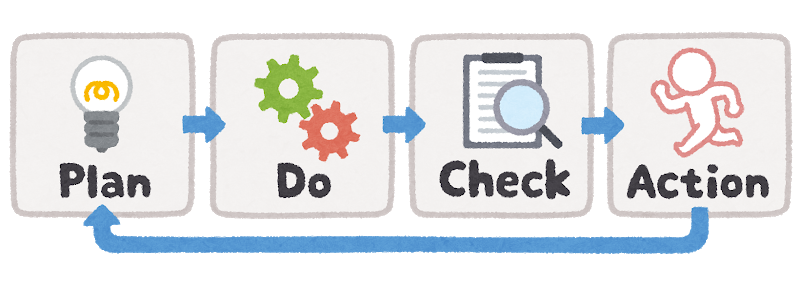
\includegraphics[width=.6\textwidth]{../img/irasutoya_pdca}\ppagenote{PDCA icon from \url{https://www.irasutoya.com}}
  \end{center}
\end{frame}

\begin{frame}{Motivation}
  In my years in Tsukuba, I have seen students commit the same errors many times in their presentations:
  \bigskip

  \begin{itemize}
    \item Experiments that do not control for noise factors;
    \item Comparative experiments that are not fair;
    \item Experiments that are not reproducible;
    \item Experiments that are not falsifiable;
    \item Unclear experimental conditions and assumptions;
  \end{itemize}
  \bigskip

  \structure{The final result is the same}: The experimental result does not support the conclusions of the student.
\end{frame}

\begin{frame}{Motivation}{These problems are not limited to students}

  \begin{itemize}
    \item Lack of rigorous experimentation protocol is common in Computer Science -- It is not only students that do it!
    \bigskip

    \item The situation has gotten much better in the past five years -- you will usually have a paper rejected if you don't do proper statistical analysis of your experiments;
    \bigskip

    \item But we still have a long way to go, specially compared to Bio and Psych areas;
  \end{itemize}

  \begin{block}{}
    We need to be careful to avoid a {\bf reproducibility crisis} in the computer sciences!
  \end{block}
\end{frame}

\begin{frame}{What will you learn in this course?}
  \begin{itemize}
    \item How to design experiments for your own research;\bigskip

    \item How to analyse your own experimental data in a robust way;\bigskip

    \item How to read and criticize scientific experiments for robustness;\bigskip
  \end{itemize}
  \bigskip

  If your research topic requires using computational experiments to show the efficacy of your proposed methods, this course will be specially useful for you.
\end{frame}
\begin{frame}{Course Topics}
  \begin{itemize}

    \item What is an experiment:
    \begin{itemize}
      \item Characteristics of a robust, reliable, reproducible experiment;
      \item How to design an experiment to answer a scientific question;
      \item Pitfalls to avoid when designing an experiment;
    \end{itemize}\bigskip

    \item Statistical tools for analyzing experimental data:
    \begin{itemize}
      \item Basic statistics for data analysis and visualization;
      \item Statistical Inference
      \item Statistical testing for single, paired, and multiple sample testing;
    \end{itemize}
  \end{itemize}
\end{frame}


\section{Course Materials}
\begin{frame}{Course Materials}
  The materials of this course can be found on the "manaba" system: \url{https://manaba.tsukuba.ac.jp/ct/course_1354290}. If you are a member of the University of Tsukuba, but not enrolled in this course, you can still access the manaba course using the self registration code: 5685116.
  \bigskip

  If manaba is not available, or you are not part of University of Tsukuba, you can access most of the materials on the github repository for this course: \url{https://caranha.github.io/ExperimentDesignCS/}. However, report submission and some of the recommended readings are only available through manaba.
\end{frame}

\begin{frame}{Course Materials}{Lecture Notes}
  The main materials for this course are these lecture notes.
  Make sure to read them and ask questions if anything is unclear!
  \vspace{1cm}

  \begin{columns}
    \column{0.8\textwidth}
    The lecture notes were produced based on the "Design and Analysis of Experiments" material produced by Felipe Campelo. You can reach the original lecture notes on: \url{https://github.com/fcampelo/Design-and-Analysis-of-Experiments}

    \column{0.2\textwidth}
    \hfill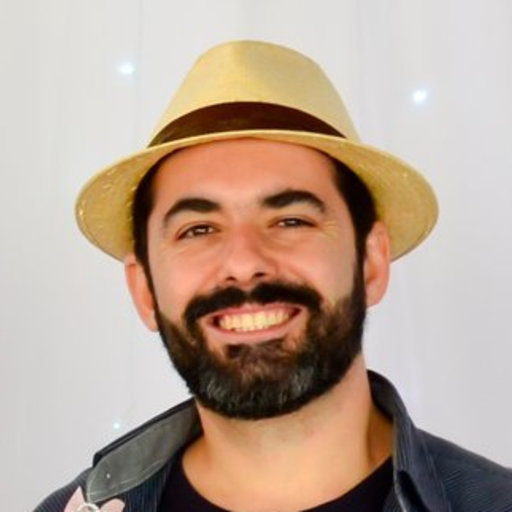
\includegraphics[width=1\textwidth]{../img/Felipe_Campelo}
  \end{columns}
  \vspace{1cm}

  All good ideas are thanks to Felipe (and other contributors) all errors are my own :-) (Please submit errors as github issues!)
\end{frame}

\begin{frame}{Course Materials}{Books and Links}
  \begin{columns}
    \column{0.2\textwidth}
    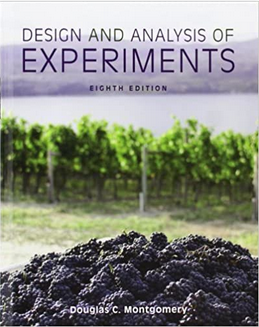
\includegraphics[width=1\textwidth]{../img/DesignAnalysis_book}
    \column{0.8\textwidth}
    Many topics in this course are explored in much more depth on "Design and Analysis of Experiments", by Douglas C. Montgomery.
    \ppagenote{"Design and Analysis of Experiments" book cover image from Amazon.}
  \end{columns}
  \vspace{1cm}

  In manaba there will be a much larger list of resources for
  extra study available. Make sure to check it out!
\end{frame}

\begin{frame}{Course Limitations}
  \hfill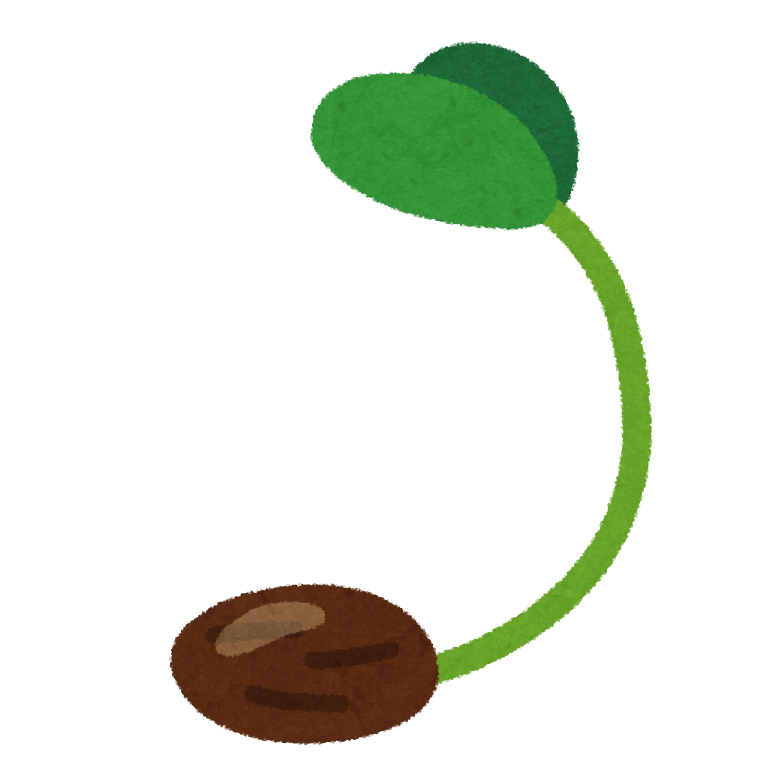
\includegraphics[width=0.2\textwidth]{../img/irasuto_sprout}
  \ppagenote{Sprout image from \url{https://www.irasutoya.com}}\\

  This course is just an {\bf introduction} to the ideas and tools of statistical analysis. Each experiment is different, and the specifics of your experiment might require different tools that are not described here.\bigskip

  I expect that students will see this course as a \structure{starting point} to get familiar with the basic concepts of statistical testing, and look for more specific information for their unique needs.
\end{frame}


\section{Lectures and Evaluation}

\begin{frame}{Weekly Schedule}
  The course is composed of {\bf regular lectures} and {\bf review and discussion lectures}.\bigskip

  \begin{itemize}
    \item {\bf Regular lectures}: Download the Lecture Notes from manaba or github. See the video link for a detailed discussion. Study the recommended resources.\bigskip

    \item {\bf Review and discussion}: Lecture will take place using an online meeting tool (TBD). Students may ask questions and receive feedback about their reports.
  \end{itemize}\bigskip

  Use the "Forums / 掲示板" area on manaba to ask questions too!
\end{frame}

\begin{frame}{Course Calendar}
\begin{itemize}
  \item 5/1 : Introduction (Today)
  \item 5/8 : Point and Interval Indicators
  \item 5/15 : Inference Testing I - {\bf Deadline Report 1}
  \item 5/22 : Inference Testing II
  \item 5/28 : Inference Testing III
  \item \alert{6/5 : Case Study, Review and Discussion}
  \item 6/12 : Power Analysis and Sample Size - {\bf Deadline Report 2}
  \item 6/19 : Anova and Post-hoc testing
  \item 6/26 : Blocking and Parameter Selection
  \item \alert{6/27 : Case Study, Review and Discussion}
  \item 7/3 : {\bf Deadline Report 3}
\end{itemize}
\end{frame}

\begin{frame}{Grading}
  The grading of this course is based on three reports. (No final examination).
  \bigskip

  \begin{itemize}
    \item \structure{Report 1}: Submit before lecture 3 (30\%)
    \item \structure{Report 2}: Submit before lecture 7 (30\%)
    \item \structure{Report 3}: Submit 1 week after lecture 10 (40\%)
  \end{itemize}
  \bigskip

  Each report is a "mini paper", including an experiment description, data acquisition, data analysis and discussion of the results.It must use the techniques and ideas introduced in this course.
\end{frame}

\begin{frame}{Report requirements}
  \begin{itemize}
    \item The reports must be submitted in English;\medskip

    \item Besides the report text (in PDF format), the reports must include all information necessary for reproducing the analysis.
    \begin{itemize}
      \item Data aquisition protocol and/or code for data generation;
      \item Code for reproducing statistical analysis and figures, including data files\footnote{It is easy to provide this data if you generate your report using R Markdown, but this is not reqired};
    \end{itemize}\medskip

    \item The report will be graded by the correctness of the analysis, and the quality of the discussion, but {\bf not} on the results of the experiments (negative results are ok!)\medskip

    \item You are encouraged (not required) to write reports based on your research!
  \end{itemize}

\end{frame}

\section{Others}
\begin{frame}{Computer Science English Program (CSE)}
  The (CSE) supports a master degree fully in English. If you plan to take many classes in English, I encourage you to enroll in the this program.
  \bigskip

  \begin{center}
    Send an e-mail with your name (Roman letters and Kanji) and student ID to\\
    \structure{s-g30@cs.tsukuba.ac.jp}
  \end{center}
  \bigskip

  For more information, see the orientation material at the
  "New Student Orientation" course on manaba (xx20011-002).
\end{frame}

\begin{frame}{About the Lecturer}
  \begin{columns}
    \column{0.4\textwidth}
    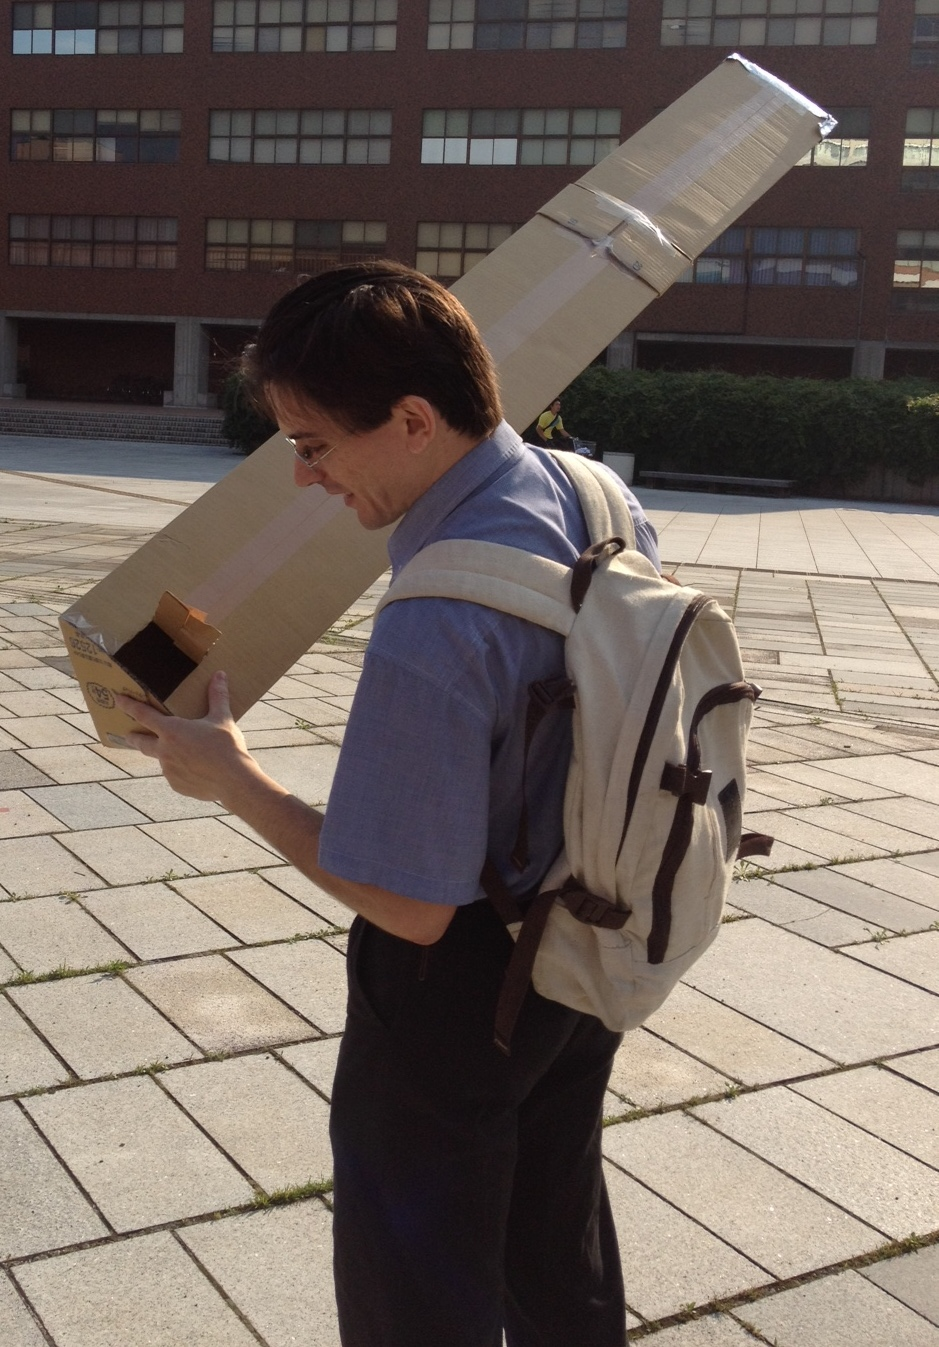
\includegraphics[width=1\textwidth]{../img/pinhole}
    \column{0.6\textwidth}
    {\small
    \begin{itemize}
      \item \structure{Name:} Claus Aranha;
      \item \structure{Country:} Brazil;
      \item \structure{Research Topics:}
      \begin{itemize}
        \item Evolutionary Algorithms;
        \item Artificial Life;
      \end{itemize}
      \item \structure{Hobbies:}
      \begin{itemize}
        \item Game Programming;
        \item Astronomy;
      \end{itemize}
        \medskip

      \item \structure{webpage:}\\ {\smaller \url{http://conclave.cs.tsukuba.ac.jp}}
    \end{itemize}
    }
  \end{columns}
\end{frame}

\section{Backmatter}
\begin{frame}{About these Slides}
  These slides were made by Claus Aranha, 2020. You are welcome to copy, re-use and modify this material.
  \bigskip

  These slides are a modification of "Design and Analysis of Experiments (2018)" by Felipe Campelo, used with permission.
  \bigskip

  Individual images in some slides might have been made by other
  authors. Please see the references in each slide for those cases.
\end{frame}

\begin{frame}[allowframebreaks]{Image Credits}
  \printnotes
\end{frame}

\end{CJK}
\end{document}
